\chapter{Higgs boson reconstruction in the Higgsino search}
\label{app:higgs}

This appendix discusses the approaches that have been tested for the reconstruction of the 
candidate Higgs bosons for the Higgsino search described in Chapter \ref{chap:ewk_prod}. 
The signal events considered in this appendix are those where both Higgs bosons decay to a $b\bar{b}$ pair. 
As already discussed in Section \ref{sec:ewk:sigbkg}, the four jets selected to reconstruct the two Higgs bosons 
are selected with the following criteria:

\begin{itemize}
\item If there are exactly four $b$-tagged jets in the event, those are used.
\item If there are more than four $b$-tagged jets, the selected ones are the four $b$-tagged jets with highest \pt.
\item If there are less than four $b$-tagged jets, the selected ones are the $b$-tagged jets and the non-tagged jets with highest \pt.
\end{itemize}

The fraction of events where this choice selects the four correct jets is shown in Figure \ref{fig:h_reco_match_possible} 
for signals with different Higgsino masses. 
Figure \ref{fig:h_reco_match_possible} shows also the fraction of events where it should be possible to select the four correct jets, 
which corresponds to requiring four jets with \pt $>$25 GeV  matched in dR$<$0.3 with the 4 b-quarks coming from the two Higgs bosons.

\begin{figure*}[h]
\centering
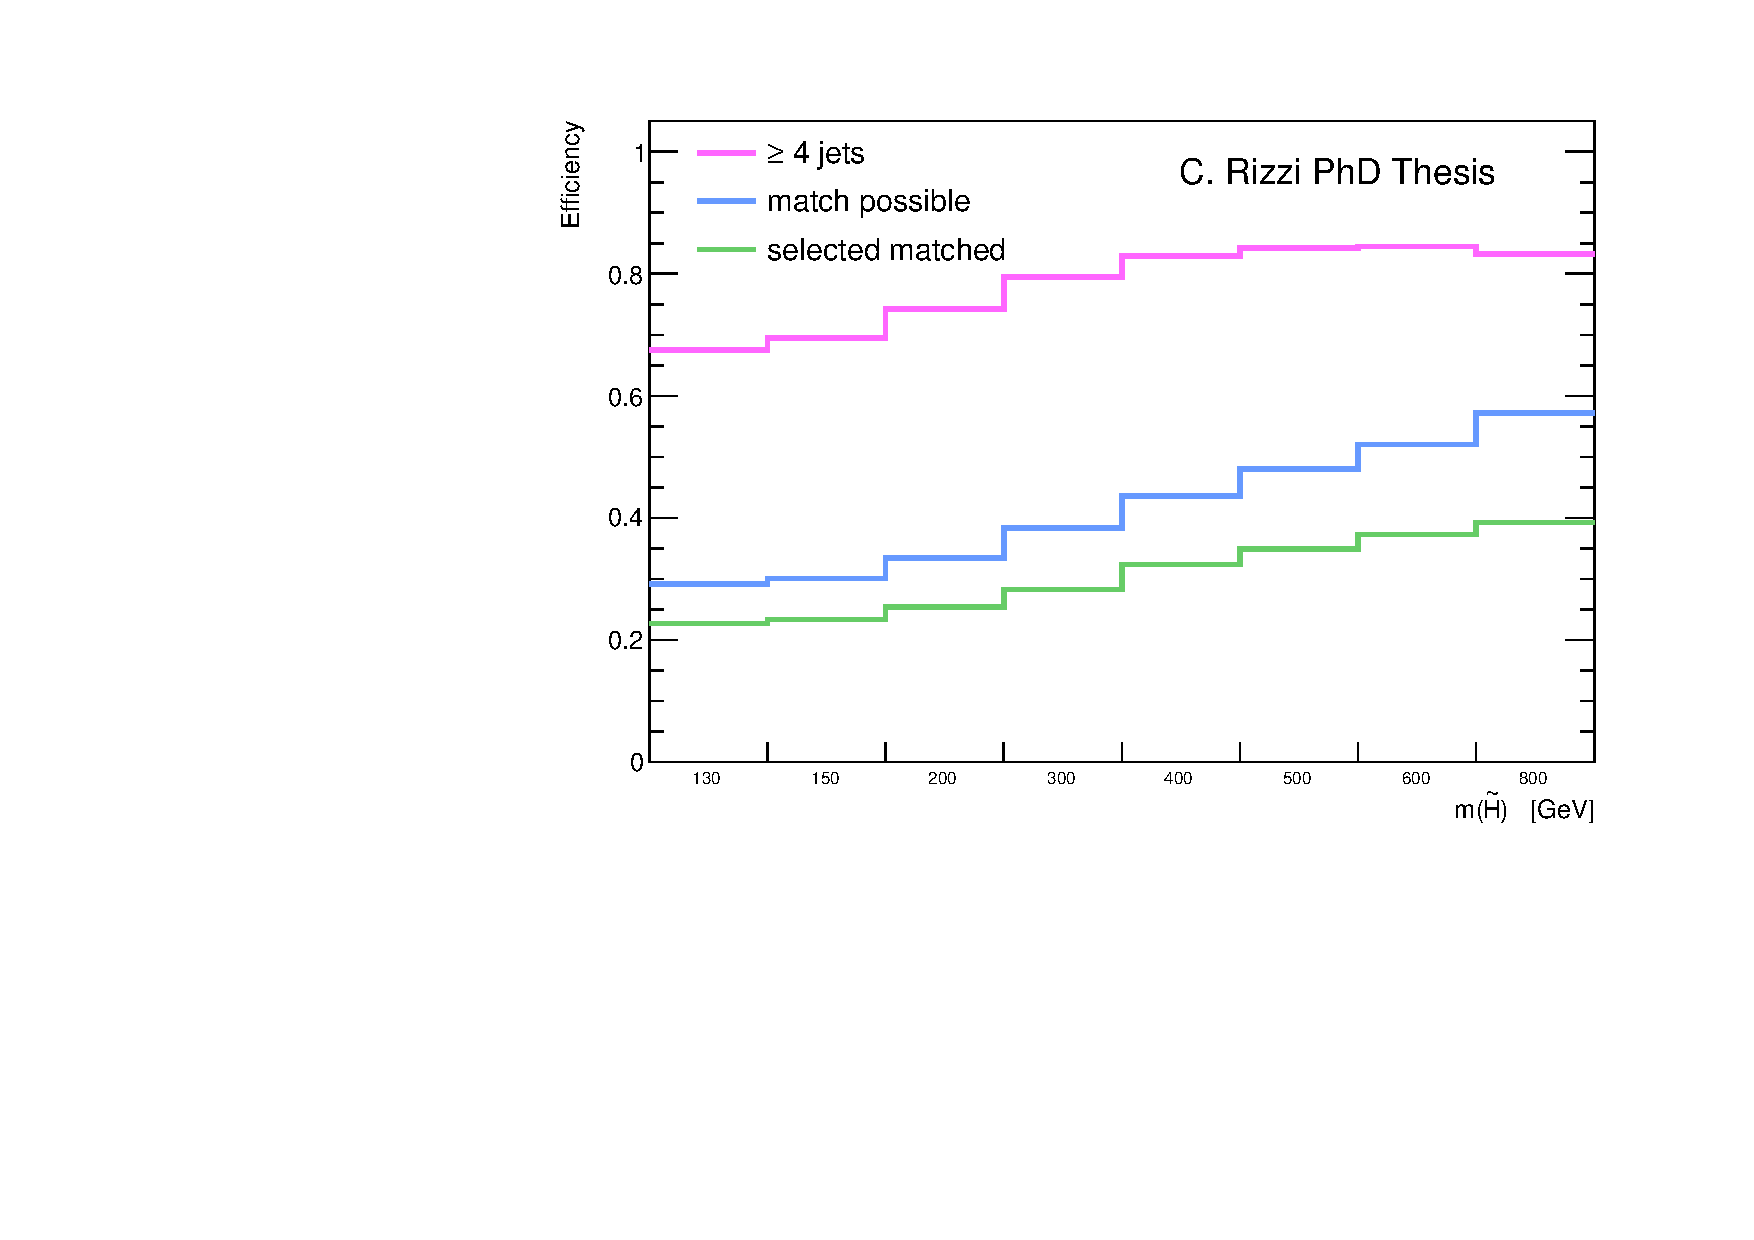
\includegraphics[width=0.7\textwidth]{figures/h_reco/match_possible.pdf}
\caption{Fraction of events where the algorithm described in the text selects the correct jets.}
\label{fig:h_reco_match_possible}
\end{figure*}

Once the four jets are selected, 
different algorithms to group them into pairs (each one corresponding to one of the two Higgs boson candidates) 
are compared: 

\begin{description}
%\item[115] Choose the pairing in which one of the masses is closer to 115 GeV (the value of 115 has been determined by signal studies showing that it was the peak of the reconstructed mass for the correct pairing).
\item[min-diff] Minimize the difference between m($h_1$)  and m($h_2$), where m($h_1$) and m($h_2$) are the masses of the two boson candidates and 
m($h_1$)$>$m($h_2$).
\item[min-dR] Minimize \dRmax (defined in Section \ref{sec:ewk:sigbkg}).
\item[max-\pt] Maximize min(\pt($h_1$), \pt($h_1$)).
\end{description}

%The performance of each of these algorithms has been compared, 
%taking as reference the number of times in which a correct reconstruction is  possible. 

Figure \ref{fig:h_reco_best_match} shows the fraction of times that each of the algorithms 
described above leads to the same pairs as the true matching, with respect to the number of events in which the true matching is possible. 
For signals with a low mass the algorithms that are based on the mass information perform better, 
while at high signal masses, where the two Higgs bosons (and their decay products) are more boosted, 
the min-dR algorithm performs the best. 
Considering that the \met-based analysis focuses on signals with intermediate and high mass, 
%and that the usage of the dR algorithm allows for an easy extension also to the case of the Z boson (to look for Zh and ZZ signals), 
this algorithm was chosen and will be used in the following sections.

\begin{figure*}[h]
\centering
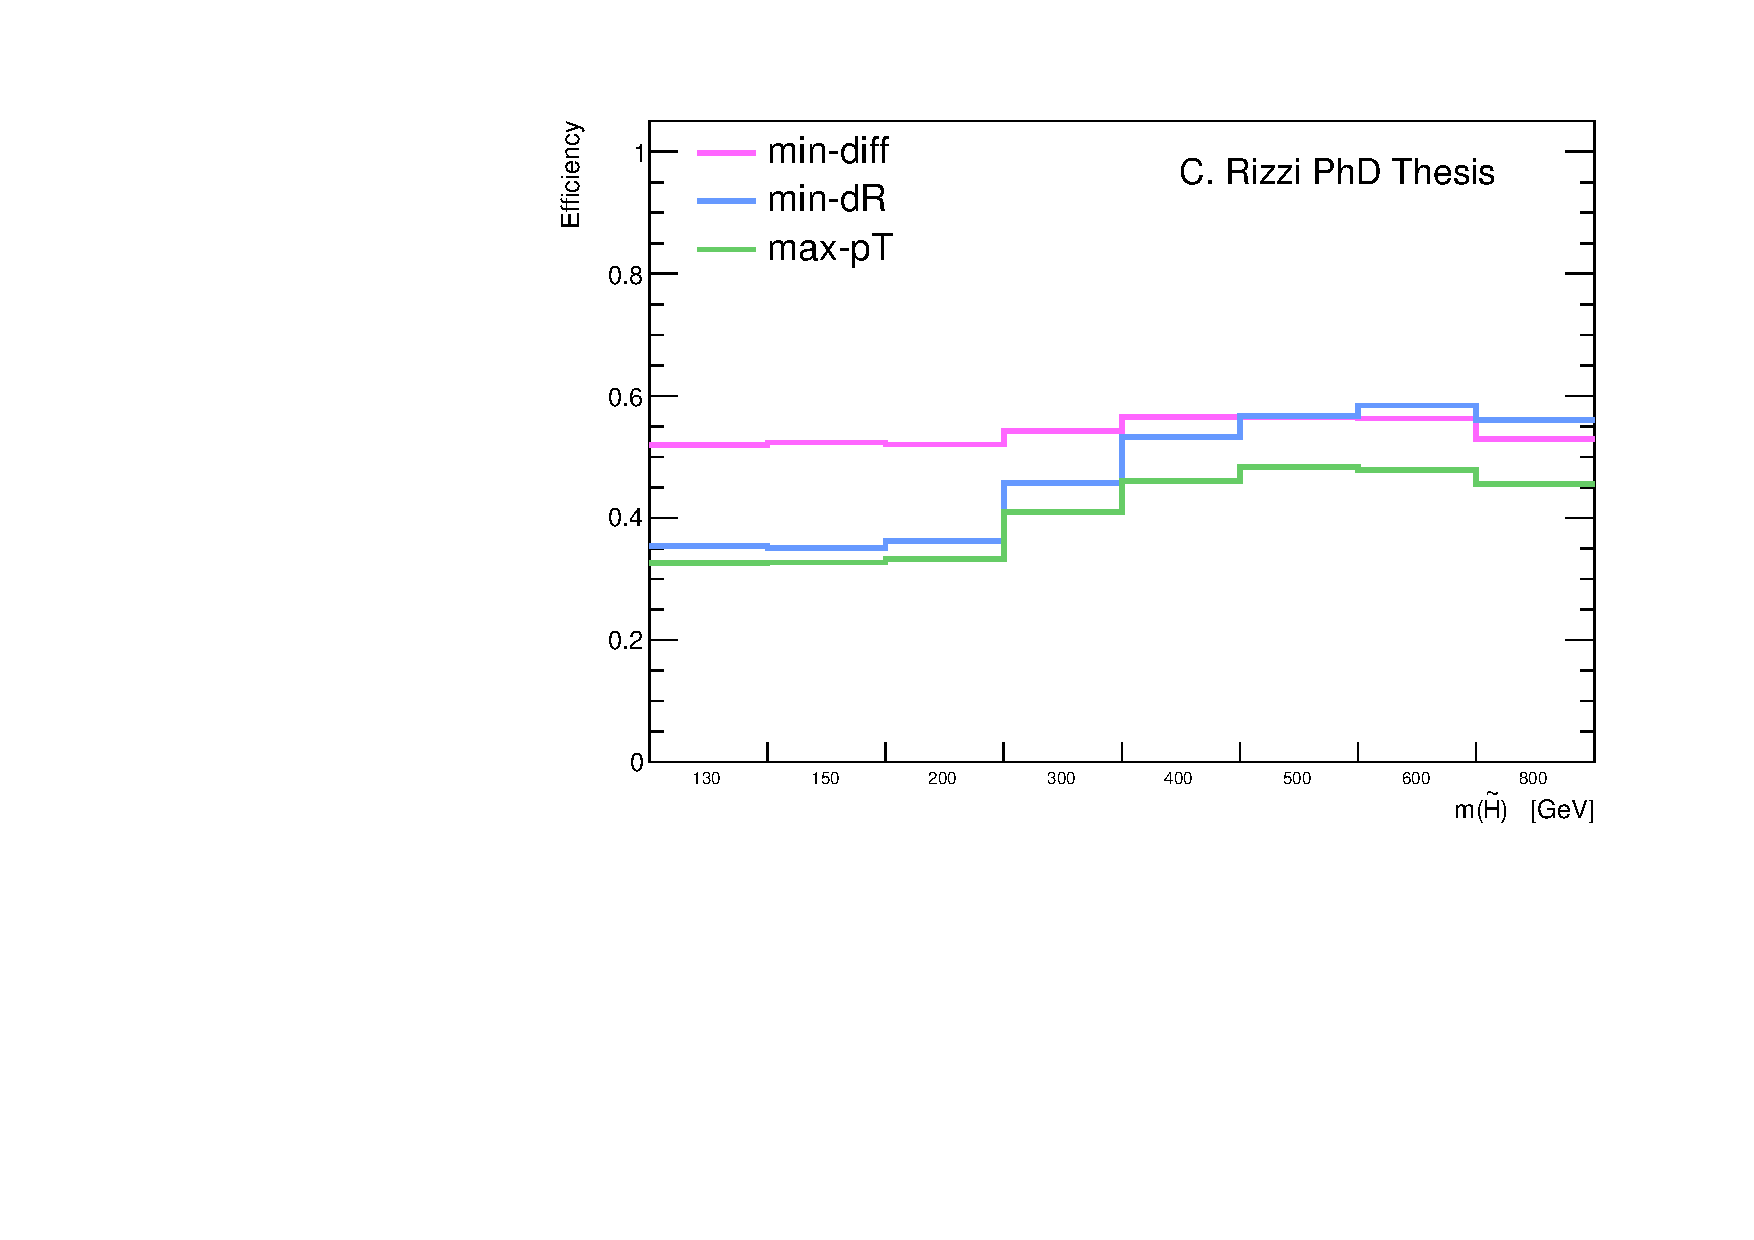
\includegraphics[width=0.7\textwidth]{figures/h_reco/best_match_if_match_possible.pdf}
\caption{Fraction of hh$\to$4b events where the reconstruction method indicated in the legend leads to the correct match. The fraction shown is with respect to the events where the correct match is possible.}
\label{fig:h_reco_best_match}
\end{figure*}

